\section{Fluxional execution model} \label{section:model}

% The compiler we present in section \ref{section:compiler} focuses on web applications that tend to follow the functional paradigm while keeping a global memory.
% Such applications are built using functions that are executed sequentially to assure the exclusivity of access on the global memory.
% This is a serious performance issue, as it avoids to leverage the parallelism of modern architectures.

% We present in this section a different execution model that isolates the memory accessible to some functions.
% This approach allows to execute these functions in parallel, hence, to benefit of the performance improvements of this parallelism.
% This execution model is close to the actor model, as the function are executed on autonomous execution units with their own isolated memory, communicating by messages.

% In this section, we present an execution model to allow the execution of functions in parallel of a main thread.
% Each parallel function is encapsulated in an autonomous execution container with its own memory.

In this section, we present an execution model to provide scalability to web applications.
% The execution of functions may dynamically be reallocated at run time depending on the load of servers.
To achieve this, the execution model provides a granularity of parallelism at the function level.
Functions are encapsulated in autonomous execution containers with their state, so as to be reallocated and executed in parallel.
This execution model is close to the actors model, as the execution containers are independent and communicate by messages.
The communications are assimilated to stream of messages, similarly to the dataflow programming model.
It allows to reason on the throughput of these streams, and to react to load increases.
% As we focus on real-time web applications, the streams of message correspond to the input stream of requests.

% This execution model is also close to the functional paradigm, as the execution container contains function to execute at each message reception.
% The function receives parameters from the input message, and sends one, or more, output streams of messages to other execution container.

The fluxional execution model executes programs written in our high-level fluxionnal language, whose grammar is presented in figure \ref{fig:flx-lang}.
An application $\bnfpn{program}$ is partitioned into parts encapsulated in autonomous execution containers named \textit{fluxions} $\bnfpn{flx}$.
In the following paragraphs, we present the \textit{fluxions}.
Then we present the messaging system to carry the communications between \textit{fluxions}.
Finally, we present an example application using this execution model.

\subsection{Fluxions}
% $\bnfpn{flx}$
% $\bnfpn{id}$
% $\bnfpn{fn}$
% $\bnfpn{ctx}$
% $\bnfpn{fn}$
% $\bnfpn{stream}$
% $\bnfpn{dest}$

% The fluxional execution model manages and invokes fluxions.
A \textit{fluxion} $\bnfpn{flx}$ is named by a unique identifier $\bnfpn{id}$ to receive messages, and might be part of one or more groups indicated by tags $\bnfpn{tags}$.
A \textit{fluxion} is composed of a processing function $\bnfpn{fn}$, and a local memory called a \textit{context} $\bnfpn{ctx}$.
% Figure \ref{fig:flx-lang} presents the fluxionnal language we designed to express fluxions.
% The function encapsulated by a \textit{fluxion} consumes an input stream and generates one or more outputs streams.
At a message reception, the \textit{fluxion} modifies its \textit{context}, and sends messages on its output streams $\bnfpn{streams}$ to downstream \textit{fluxions}.
The \textit{context} handles the state on which a \textit{fluxion} relies between two message receptions.
% A message is composed of the recipient fluxions' names and a body.
% Message passing is unable\footnote{at reasonable costs} to replace the synchronization allowed by shared state. % and required between some of the application parts.
In addition to message passing, the execution model allows \textit{fluxions} to communicate by sharing state between their \textit{contexts}.
% To allow this synchronization when required, the execution model allows fluxions to share state between their contexts.
The fluxions that need to synchronize together are grouped with the same tag, and loose their independence.
% To assure the consistency of the shared state, all the fluxions of a group are executed sequentially.
% Though, the different groups of fluxions are executed in parallel.

There are two types of streams, \textit{start} and \textit{post}, which correspond to the nature of the rupture point yielding the stream.
We differentiate the two types with two different arrows, double arrow (\texttt{>>}) for \textit{start} rupture points and simple arrow (\texttt{->}) for \textit{post} rupture points.
%We differentiates the two types with two different arrows, double arrow ($\twoheadrightarrow$ or \texttt{>>}) for \textit{start} rupture points and simple arrow ($\to$ or \texttt{->}) for \textit{post} rupture points.
The two types of rupture points are further detailed in section \ref{section:compiler:analyzer:rupture}.


% Fluxions are executed on an event-loop with an isolated heap ; it is a \textit{Node.js} instance.
% We propose to stretch the execution of an application by distributing the fluxions on different event-loops.
% But the distribution is limited by the dependencies between fluxions.
% All the fluxions of a group need to be gathered on the same event-loop.
% Indeed, each event-loop assures the exclusivity of access to the state: only one fluxion is executed at once.
% Consequently, the more fluxions are gathered on an event-loop, the less time fraction each fluxion can use without impacting the throughput.

%These groups represent the graph of state communications between fluxion.
%Hence, this graph indicates the states that are limiting the parallelism.


% A fluxion receiving and sending heap reference can be stateless, hence replicated.
% However, because it share references, it needs to be on the same group than other another fluxions (think about req / res).
% If all the fluxion of a group are stateless, they can be replicated exactly like if it was a single fluxion. 








% It is the target for our compiler.
\begin{figure}
\vspace{-0.6\baselineskip}
\begin{bnf*}
  \bnfprod{program}    {\bnfpn{flx} \bnfor \bnfpn{flx} \bnfsp \bnftd{eol} \bnfsp \bnfpn{program}}\\
  \bnfprod{flx}        {\bnfts{\texttt{flx}} \bnfsp \bnfpn{id} \bnfsp \bnfpn{tags} \bnfsp \bnfpn{ctx} \bnfsp \bnftd{eol} \bnfsp \bnfpn{streams} \bnfsp \bnftd{eol} \bnfsp \bnfpn{fn}}\\
  % \bnfprod{tags}       {\bnfts{\bnfpn{id}} \bnfor \bnfpn{id} \bnfsp \bnftd{eol} \bnfsp \bnfpn{tags} \bnfor \bnftd{empty string}}\\
  \bnfprod{tags}       {\bnfts{\texttt{\&}} \bnfsp \bnfpn{list} \bnfor \bnftd{empty string}}\\
  \bnfprod{streams}    {\bnfts{\texttt{null}} \bnfor \bnfpn{stream} \bnfor \bnfpn{stream} \bnfsp \bnftd{eol} \bnfsp \bnfpn{streams}}\\
  \bnfprod{stream}     {\bnfpn{type} \bnfsp \bnfpn{dest} \bnfsp [\bnfpn{msg}]}\\
  \bnfprod{dest}       {\bnfpn{list}}\\
  \bnfprod{ctx}        {\bnfts{\texttt{\{}} \bnfpn{list} \bnfts{\texttt{\}}}}\\
  \bnfprod{msg}        {\bnfts{\texttt{[}} \bnfpn{list} \bnfts{\texttt{]}}}\\
  \bnfprod{list}       {\bnfpn{id} \bnfor \bnfpn{id} \bnfsp \bnfts{,} \bnfsp \bnfpn{list}}\\
  \bnfprod{type}         {\bnfts{\texttt{>}\texttt{>}} \bnfor \bnfts{\texttt{-}\texttt{>}}}\\
  \bnfprod{id}         {\bnftd{Identifier}}\\
  \bnfprod{fn}         {\bnftd{imperative language and stream syntax}}\\
\end{bnf*}
\vspace{-2.5\baselineskip}
\caption{Syntax of a high-level language to represent a program in the fluxionnal form}
\label{fig:flx-lang}
\end{figure}

\subsection{Messaging system}

% In a distributed approach, the messages between fluxions would be carried over a distributed message broker.
% However this execution model is only a simulation of a distributed execution environement.
% We simplify the distributed message broker with a master message queue to centralize communication between workers, though, each worker has its own local message queue.
% The messaging system is the core of the execution model.
% It carries messages and invokes fluxions at reception.
% The messaging system sends messages to the worker hosting the destination fluxion.
% Locally, the master worker hosts fluxions that need access to the external network or the global memory.
% Using a message queue allows to execute multiple processing chains fairly and concurrently, without difference in scheduling local messages, or network messages.

The messaging system assures the stream communications between fluxions.
It carries messages based on the names of the recipient fluxions.
After the execution of a fluxion, it queues the resulting messages for the event loop to process.
% The messages are queued for the event-loop to execute the associated fluxions sequentially.

% The execution model allows each group of fluxions to be executed on a remote event-loop.
% Therefore, some messages need to be send to remote event-loops.
% When processing a message, if the destination fluxion is local, the messaging system immediately invokes the fluxion with the message, if it is on a remote event-loop, the messaging system sends the message to be queued on the remote event-loop.



% The messaging system carries messages from one event-loop to the other, and assure that the message is queued on the event-loop executing the destination fluxion.

% If two fluxions share the same name, it would lead to a conflicting situation for the messaging system.

% This registration associates a processing function with a unique name and an initial \textit{context}.
% The registration is done by calling \texttt{register(<name>, <fn>, <context>)}, \circled{1}.
% A fluxion can dynamically register other fluxions

The execution cycle of an example fluxional application is illustrated in figure \ref{fig:MesSys}.
Circles represent registered fluxions.
The source code for this application is in listing \ref{lst:source} and the fluxional code for this application is in listing \ref{lst:fluxional}.
The fluxion \textit{reply} has a context containing the variable \texttt{count} and \texttt{tem\-plate}.
The plain arrows represent the actual message paths in the messaging system, while the dashed arrows between fluxions represent the message streams as seen in the fluxionnal application.
% The streams between workers are serialized.

% To assure the consistency of their shared contexts, all the fluxions grouped with the same tag are executed sequentially and share the same message queue.
% Though, the different groups of fluxions are executed in parallel with different event queues.

% This first message represents the incoming of a request from a user.
The \textit{main} fluxion is the first fluxion in the flow.
When the application receives a request, this fluxion triggers the flow with a \texttt{start} message containing the request, \circled{2}.
This first message is to be received by the next fluxion \textit{handler}, \circled{3} and \circled{4}.
The fluxion \textit{handler} sends back a message, \circled{5}, to be enqueued, \circled{6}.
The system loops through steps \circled{3} through \circled{6} until the queue is empty.
This cycle starts again for each new incoming request causing another \texttt{start} message.

\begin{figure}[h!]
  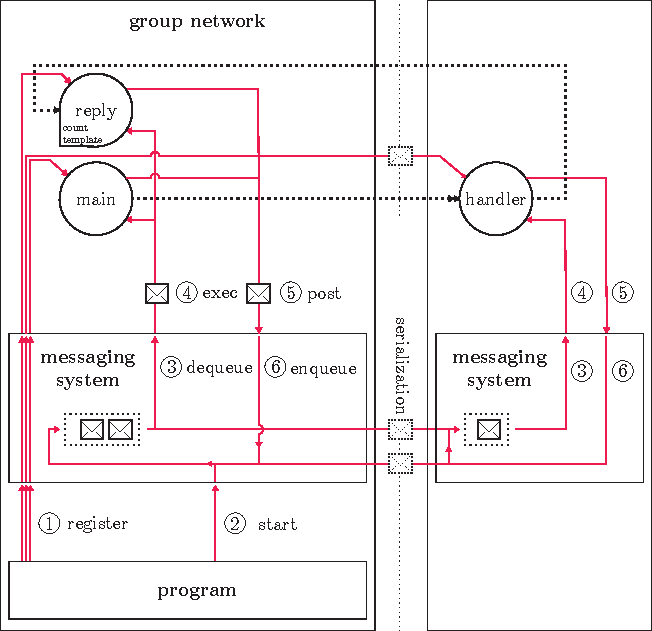
\includegraphics[width=\linewidth]{resources/schema-message.pdf}
  \caption{The fluxionnal execution model in details}
  \label{fig:MesSys}
\end{figure}

% Algorithms \ref{alg:parcours} and \ref{alg:traitement} describe the behavior of the messaging system after the \texttt{start} function invocation.

% \begin{algorithm}
% \caption{Message queue walking algorithm}
% \label{alg:parcours}
% \begin{algorithmic}
% \Function{loopMessage}{\null}
% \While{$msg$ \textbf{presents in} $msgQueue$}
% \State $msg \gets$ \Call{dequeue}{\null} \Comment{\circled{3}}
% \State \Call{ProcessMsg}{$msg$}
% \EndWhile
% \EndFunction
% \end{algorithmic}
% \end{algorithm}

% \begin{algorithm}
% \caption{Message processing algorithm}
% \label{alg:traitement}
% \begin{algorithmic}
% \Function{processMsg}{$msg$}
% \For{$dest$ \textbf{in} $msg.dest$}
% \State $worker \gets lookup(dest)$
% \State \Call{worker.send}{$fluxion, msg.body$} \Comment{\circled{4}}
% % \State $message \gets$ \Call{exec}{$fluxion, msg.body$} \Comment{\circled{4} \& \circled{5}}
% % \State \Call{enqueue}{$message$} \Comment{\circled{6}}
% \EndFor
% \EndFunction
% \end{algorithmic}
% \end{algorithm}

\subsection{Service example}

To illustrate the fluxional execution model, and the compiler, we present in listing \ref{lst:source} an example of a simple web application.
This application reads a file, and sends it back along with a request counter.

\begin{code}[js,
  caption={Example web application},
  label={lst:source}]
var app = require('express')(),
    fs = require('fs'),
    count = 0;

app.get('/', function handler(req, res){
  fs.readFile(__filename, function reply(err, data) {
    count += 1;
    res.send(err || template(count, data));
  });
});

app.listen(8080);
\end{code}

% The original source code of this application is available in listing \ref{lst:source}\footnote{The listings are also available on github\cite{flx-example}.}.
% In this example application, some points are worth noticing.
The \texttt{handler} function, line 5 to 11, receives the input stream of request.
The \texttt{count} variable at line 3 increments the request counter.
This object needs to be persisted in the fluxion \textit{context}.
The \texttt{template} function formats the output stream to be sent back to the client.
The \texttt{app.get} and \texttt{res.send} functions, respectively line 5 and 8, interface the application with the clients.
And between these two interface functions is a chain of three functions to process the client requests : \texttt{app.get} $\to$ \hspace{-1.4em} $\to$ \texttt{handler} $\to$ \texttt{reply}.
This application is transformed into the high-level fluxionnal language in listing \ref{lst:fluxional} which is illustred in Figure \ref{fig:MesSys}.
% We expect a similar result with the compiler described in section \ref{section:compiler}.
% Horizontal dashed lines show virtual transmission of messages between fluxions although they all go through the messaging system.

% \begin{figure}[h!]
%   \includegraphics[width=\linewidth]{ressources/flux.pdf}
%   \caption{Fluxions chain manually extracted from the example application}
%   \label{fig:fluxions}
% \end{figure}

\begin{code}[flx, caption={Example application expressed in the high-level fluxional language}, label={lst:fluxional}]
flx main & network
>> handler [res]
  var app = require('express')(),
      fs = require('fs'),
      count = 0;

  app.get('/', >> handler); //@\label{lst:fluxional-streamtohandler}@
  app.listen(8080);

flx handler
-> reply [res]
  function handler(req, res) {
    fs.readFile(__filename, -> reply); //@\label{lst:fluxional-readfile}@
  }

flx reply & network {count, template}
-> null
  function reply(error, data) {
    count += 1; //@\label{lst:fluxional-counter}@
    res.send(err || template(count, data)); //@\label{lst:fluxional-ressend}@
  }
\end{code}

The application is organized as follow.
The flow of requests is received from the clients by the fluxion \texttt{main}, it continues in the fluxion \texttt{handler}, and finally goes through the fluxion \texttt{reply} to be sent back to the clients.
The fluxions \texttt{main} and \texttt{reply} have the tag \texttt{network}.
This tag indicates their dependency over the network interface, because they  received the response from and send it back to the clients.
The fluxion \texttt{handler} doesn't have any dependencies, hence it can be executed in parallel.

The last fluxion, \texttt{reply}, depends on its context to holds the variable \texttt{count} and the function \texttt{template}.
It also depends on the variable \texttt{res} created by the first fluxion, \texttt{main}.
This variable is carried by the stream through the chain of fluxion to the fluxion \texttt{reply} that depends on it.
This variable holds the references to the network sockets.
It is the variable the group \texttt{network} depends on.

Moreover, if the last fluxion, \texttt{reply}, did not relied on the variable \texttt{count}, the group \texttt{network} would be stateless.
The whole group could be replicated as many time as needed. % to cope with the incoming traffic.

This execution model allows to parallelize the execution of an application.
Some parts are arranged in pipeline, like the fluxion \texttt{handler}, some other parts are replicated, as could be the group \texttt{network}.
This parallelization improves the scalability of the application.
Indeed, as a fluxion contains its state and expresses its dependencies, it can be migrated.
It allows to adapt the number of fluxions per core to adjust the resource usage in function of the desired throughput.


% Fluxions with no state could be replicated to make data parallelism, additionally to the pipeline parallelism.

Our goal, as described in the introduction, is not to propose a new programming paradigm with this high-level language but to automate the architecture shift.
We present the compiler to automate this architecture shift in the next section.